\section{Auswertung}
\label{sec:Auswertung}

\begin{align}
m_\mathrm{k}&=(5,833 \pm 0,235)\cdot 10^{-3} \si{\kilogram} \\
2R_\mathrm{k}&=(51,03 \pm 0,02) \si{\milli \meter} \\
\theta_\mathrm{k} &= 2.25 \cdot 10^‚{-6}   \si{\kilogram \meter}^2 \\
N &= 80 \\
R_\mathrm{Spule}&=72 \si{\milli \meter} \\
\end{align}

Das Trägheitsmoment der Kugel beträgt $\theta_\mathrm{Kugel} = \frac{2m_\mathrm{k} R_\mathrm{k}^2}{5} = (1,532 \pm 0,0013)\cdot 10^{-4} \si{\kilogram \meter}^2$. Das Gesamtträgheitsmoment ergibt sich durch die Addition des Trägheitsmoments der Halterung $\theta_\mathrm{k}$ und $\theta_\mathrm{Kugel}$.
\begin{equation}
  \theta_\mathrm{ges}=(1,545 \pm 0,0013)\cdot 10^{-4} \si{\kilogram \meter}^2
\end{equation}
\subsection{Messung ohne B-Feld}

\begin{table}
  \caption{Periodendauer mit Schraube parallel zum Draht.}
  \centering
  \label{tab:par}
  \begin{tabular}{c}
    \toprule
    $T/s$ \\
    19,798 \\
    19,795 \\
    19,811 \\
    19,821 \\
    19,803 \\
    19,806 \\
    19,817 \\
    19,820 \\
    19,805 \\
    19,808 \\
    19,816 \\
    19,819 \\
    \bottomrule
    \end{tabular}
    \end{table}


    \begin{table}
      \caption{Periodendauer mit Schraube senkrecht zum Draht in Nord-Süd Richtung.}
      \centering
      \label{tab:senk}
      \begin{tabular}{c}
        \toprule
        $T/s$ \\
        19,395 \\
        19,395 \\
        19,403 \\
        19,408 \\
        19,391 \\
        19,425 \\
        19,409 \\
        19,409 \\
        19,403 \\
        19,409 \\
        \bottomrule
        \end{tabular}
        \end{table}

Die Messwerte zur Periodendauer bei parallel zum Draht ausgerichtetem Magnetn befinden sich in Tabelle \ref{tab:par} und die zu senkrecht zum Draht ausgerichteten Magneten in Tabelle \ref{tab:senk}.
Es ergeben sich folgende Mittelwerte für die Periodendauer:
\begin{align}
  T_\mathrm{parallel}&=(19,810 \pm 0,003) \si{\second} \\
  T_\mathrm{senkrecht}&=(19,4047 \pm 0,0090) \si{\second} \\
\end{align}
Es fällt auf, dass die Periodendauer bei Nord-Süd Ausrichtung kürzer ist.


\subsection{Bestimmung des Schubmoduls}

\begin{table}
  \caption{Messwerte zur Bestimmung der Maße des Drahtes.}
  \centering
  \label{tab:draht}
  \begin{tabular}{c c c}
    \toprule
    $L_1 / \si{\meter}$ & $L_2 / \si{\meter}$ & $2R / \si{\milli \meter}$ \\
0,617 & 0,0045 & 0,203 \\
0,615 & 0,0045 & 0,204 \\
0,616 & 0,0046 & 0,204 \\
/ & / & 0,202 \\
/ & / & 0,203 \\
/ & / & 0,200 \\
\bottomrule
\end{tabular}
\end{table}

In Tabelle \ref{tab:draht} sind die Messwerte zur Länge und zum Durchmesser des Drahtes dargestellt. $L_1$ ist dabei die Länge des Drahtes von der vom Justierrad zum Spiegel und $L_2$ die vom Spiegel bis zur Kugel. Die Gesamtlänge $L$ ist die Summe von $L_1$ und $L_2$.
Die Mittelwerte lauten:
\begin{align}
  2R&=(0,2027 \pm 0,0006)\si{\milli\meter} \\
  L_1&=(0,616 \pm 0,0006)\si{\meter} \\
  L_2&=(0,0453 \pm 0,0003) \si{\meter}.
\end{align}

Das Schubmodul lässt sich mit Hilfe folgender Formel berechnen:
\begin{equation}
  G = \frac{16\pi m_\mathrm{k} R_\mathrm{k}^2 L}{5T^2 R^4}.
\end{equation}

Somit ist $G=(6,41 \pm 0,08)\cdot 10^{10} \frac{\si{\newton}}{\si{\meter}^2}$.
Dieser weicht vom Literaturwert $G_\mathrm{lit} = 8,2 \cdot 10^{10}\frac{\si{\newton}}{\si{\meter}^2}$ um $(21,8 \pm 0,009)\%$ ab.

\subsection{Bestimmung der Querkontraktionszahl}
Die Querkontraktionszahl ergibt sich aus
\begin{equation}
  \mu = \frac{E}{2G}-1.
\end{equation}
E ist gegeben beträgt $E=21 \cdot 10^{10} \frac{\si{\newton}}{\si{\meter}^2}$.
Somit folgt $\mu = (0,638 \pm 0,02)$.

\subsection{Bestimmung des Kompressionsmoduls}
 Für das Kompressionsmodul gilt
 \begin{equation}
   Q = \frac{E}{3(1-2\mu)} = (-2,5 \pm 0,4)\cdot 10^{10} \si{\pascal}.
\end{equation}


\subsection{Bestimmung der Horizotalkomponente des Erdmagnetfelds}

Unter Verwendung der Gleichungen \ref{} und \ref{} folgt
\begin{equation}
  B = \frac{4\pi^2 \theta-\mathrm{ges}}{m-\mathrm{k}T_\mathrm{senkrecht}^2} - \frac{D}{m}
\end{equation}
Die Horizontalkomponente des Erdmagnetfelds beträgt $B=(2,32 \pm 0,33)\cdot 10^{-7}\si{\tesla}$.

\subsection{Messung mit B-Feld}

Für das Magnetfeld im Innern einer Helholtz-Spule gilt
\begin{equation}
  B=\frac{4}{5}^{\frac{3}{2}} \frac{\mu_0 N I}{R_\mathrm{Spule}}
\end{equation}

mit $\mu_0=4\pi \cdot 10^{-7} \frac{\si{\newton}}{\si{\ampere}^2}$ und $I$ als Stromstärke.

\begin{table}
  \caption{Messwerte zur Periodendauer bei eingeschaltetem Magnetfeld.}
  \centering
  \label{tab:mag}
  \begin{tabular}{c c }
    \toprule
    $I/ \si{\ampere}$ & $T / \si{\second}$ \\
0,5 & 13,409 \\
0,5 & 13,417 \\
0,5 & 12,337 \\
0,5 & 13,433 \\
0,5 & 13,439 \\
0,5 & 13,439 \\
0,5 & 13,420 \\
0,5 & 13,467 \\
1 & 10,846 \\
1 & 10,868 \\
1 & 10,843 \\
1 & 10,857 \\
1 & 10,847 \\
1 & 10,855 \\
1 & 10,856 \\
1 & 10,851 \\
1,5 & 9,357 \\
1,5 & 9,346 \\
1,5 & 9,328 \\
1,5 & 9,318 \\
1,5 & 9,369 \\
1,5 & 9,338 \\
1,5 & 9,324 \\
1,5 & 9,350 \\
2 & 8,340 \\
2 & 8,321 \\
2 & 8,359 \\
2 & 8,338 \\
2 & 8,325 \\
2 & 8,338 \\
2 & 8,320 \\
2 & 8,348 \\
2,5 & 7,588 \\
2,5 & 7,544 \\
2,5 & 7,553 \\
2,5 & 7,592 \\
2,5 & 7,556 \\
2,5 & 7,551 \\
2,5 & 7,581 \\
2,5 & 7,594 \\
3,5 & 6,548 \\
3,5 & 6,558 \\
3,5 & 6,540 \\
3,5 & 6,557 \\
3,5 & 6,523 \\
3,5 & 6,571 \\
3,5 & 6,502 \\
3,5 & 6,579 \\
\bottomrule
\end{tabular}
\end{table}

Die Messwerte zur Periodendauer mit eingeschaltetem B-Feld mit verschiedenen Stromstärken sind in Tabelle \ref{tab:mag} zu finden.
Zur Bestimmung des magnetisches Moments wird $B$ gegen $\frac{1}{T^2}$ aufgetragen. Die Werte hierzu befinden sich in Tabelle \ref{tab:mag2} . Bei der angegebenen Periodendauer handelt es sich um den Mittelwert der in Tabelle \ref{tab:mag} aufgeführten Werte.

\begin{table}
  \caption{Werte für $B$ und $T$ zur Bestimmung des magnetischen Moments.}
  \centering
  \label{tab:mag2}
  \begin{tabular}{c c }
    \toprule
    $\frac{1}{T^2} / 10^{-2} \frac{1}{\si{\second}^2}$ & $B/ \si{\milli\tesla}$ \\
    0,566 & 0,5 \\
    0,849 & 0,999 \\
    1,146 & 1,499 \\
    1,397 & 1,998 \\
    1,745 & 2,498 \\
    2,333 & 3,497 \\
    \bottomrule
    \end{tabular}
    \end{table}

    \begin{figure}
      \centering
      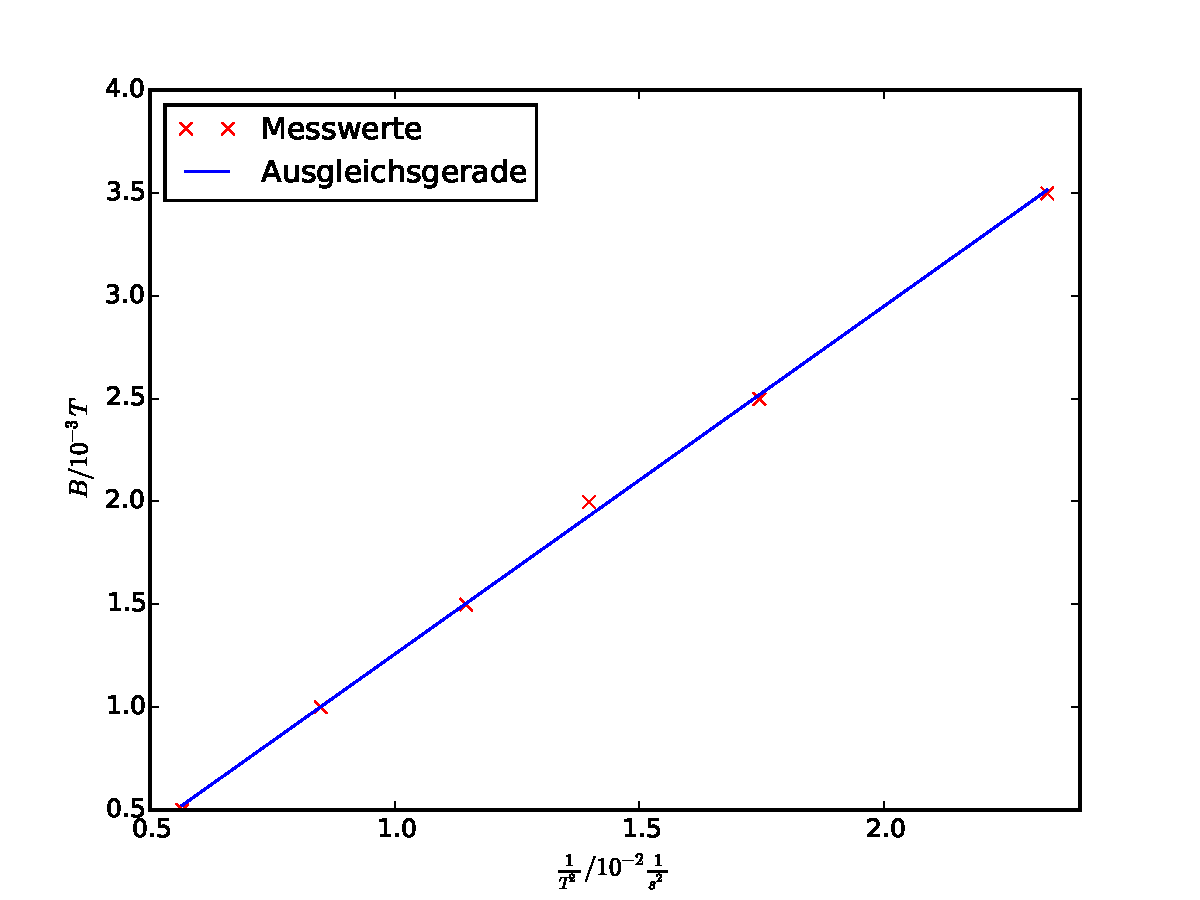
\includegraphics[width=\textwidth]{auswertung/magn-moment.pdf}
    \caption{Ausgleichsgerade zur Bestimmung des magnetischen Moments.}
      \label{fig:eckig}
    \end{figure}

    Die Gerade hat die Form $y=ax+b$. Die Parameter $a$ und $b$ haben folgende Werte:
    \begin{align}
      a&=1,692 \pm 0,027 \\
      b&= -0,0435 \pm 0,0040 \\
    \end{align}

    Mit den Gleichungen \ref{} und \ref{} folgt
    \begin{equation}
      M = 4\pi^2 \theta_\mathrm{ges} a = (0,01308 \pm 0,00017) \si{\ampere \meter}^2.
    \end{equation}
